% =====================================================================
%  CT Dose AI — short presentation (simple version)
%  pdflatex CT_Dose_AI_Presentation_simple.tex   (run twice)
%  Needs: figs/*.png
% =====================================================================
\documentclass[aspectratio=169,11pt]{beamer}

\usepackage[T1]{fontenc}
\usepackage[utf8]{inputenc}
\usepackage{helvet}\renewcommand{\familydefault}{\sfdefault}
\usepackage{amsmath,booktabs,graphicx}

\definecolor{myblue}{HTML}{2A78D6}
\definecolor{mydark}{HTML}{1A4F94}
\definecolor{mygrey}{HTML}{52514E}

\usetheme{default}
\setbeamertemplate{navigation symbols}{}
\setbeamercolor{structure}{fg=myblue}
\setbeamercolor{frametitle}{fg=mydark}
\setbeamerfont{frametitle}{size=\large,series=\bfseries}
\setbeamertemplate{frametitle}{\vspace{4mm}\hspace{2mm}\insertframetitle\par\vspace{1mm}}
\setbeamertemplate{itemize item}{\color{myblue}$\bullet$}
\setbeamertemplate{itemize subitem}{\color{myblue}--}
\setbeamertemplate{footline}{%
  \hbox{\begin{beamercolorbox}[wd=\paperwidth,ht=3ex,dp=1.5ex,leftskip=5mm,rightskip=5mm]{}%
  {\scriptsize\color{mygrey}CT Dose AI}\hfill{\scriptsize\color{mygrey}\insertframenumber\,/\,13}%
  \end{beamercolorbox}}}
\setbeamersize{text margin left=8mm,text margin right=8mm}

\title{CT Dose AI}
\subtitle{Predicting radiation dose in coronary CT angiography\\and suggesting how to lower it}
\author{Thodoris Fragos}
\date{}

\begin{document}

% ---------------- 1 ----------------
\begin{frame}[plain]
  \vspace{10mm}
  {\color{mydark}\Huge\bfseries CT Dose AI}\\[6mm]
  {\large Predicting radiation dose in coronary CT angiography,\\[1mm]
  and suggesting how to lower it}\\[12mm]
  {\color{mygrey} Thodoris Fragos \\[1mm]
  M.Sc. project \textbullet\ 50 patient examinations \textbullet\ Python}
  \vfill
\end{frame}

% ---------------- 2 ----------------
\begin{frame}{The task}
\begin{itemize}\itemsep8pt
  \item A colleague from the radiology department gave me data from \textbf{50 coronary CT scans}.
  \item For each scan we know: the patient's \textbf{BMI}, and three machine settings --- \textbf{kV}, \textbf{mAs}
  and \textbf{scan length}.
  \item We also know the two radiation dose numbers the scanner reports: \textbf{CTDIvol} and \textbf{DLP}.
\end{itemize}
\vspace{6mm}
\textbf{Two questions:}
\begin{enumerate}\itemsep6pt
  \item Can we \textbf{predict} the dose from the settings?
  \item Can we \textbf{suggest} which settings to change so the dose goes down?
\end{enumerate}
\vspace{4mm}
{\color{mygrey}BMI stays fixed: it depends on the patient, not on us.}
\end{frame}

% ---------------- 3 ----------------
\begin{frame}{The two dose numbers, in simple terms}
\begin{columns}[T]
\begin{column}{0.48\textwidth}
  \textbf{CTDIvol} (mGy)\\[2mm]
  How \emph{strong} the radiation is at each slice of the scan.\\[6mm]
  \textbf{DLP} (mGy$\cdot$cm)\\[2mm]
  The \emph{total} radiation of the examination:\\
  CTDIvol $\times$ scan length.
\end{column}
\begin{column}{0.48\textwidth}
  \textbf{In our 50 scans:}
  \begin{itemize}
    \item CTDIvol: 21 -- 105 mGy
    \item DLP: 482 -- 2393 mGy$\cdot$cm, median 1080
  \end{itemize}
  \vspace{4mm}
  Published reference level for this examination: about \textbf{400} mGy$\cdot$cm.
  \vspace{4mm}
  {\color{mygrey}So there is room to reduce the dose.}
\end{column}
\end{columns}
\end{frame}

% ---------------- 4 ----------------
\begin{frame}{First look at the data}
\begin{columns}[T]
\begin{column}{0.46\textwidth}
\begin{itemize}\itemsep6pt
  \item CTDIvol divided by mAs is almost \textbf{constant}: 0.0605 at 120 kV, 0.0894 at 140 kV.
  \item So CTDIvol is not a random pattern. It follows the physics of the machine.
  \item Five scans give about 7\% less dose per mAs. Probably a different machine setting that was not recorded.
\end{itemize}
\end{column}
\begin{column}{0.52\textwidth}
  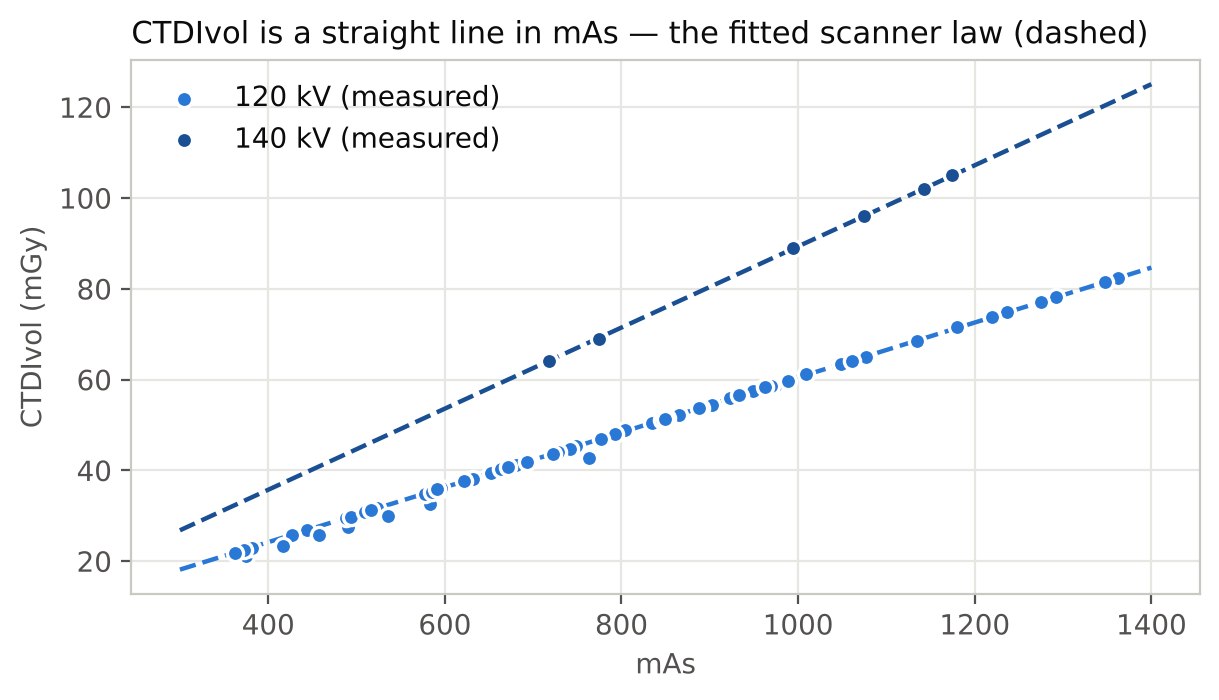
\includegraphics[width=\linewidth]{figs/f1_physics.png}
\end{column}
\end{columns}
\end{frame}

% ---------------- 5 ----------------
\begin{frame}{The model}
\vspace{2mm}
\begin{center}
\large
$\mathrm{CTDIvol} = k \times \mathrm{mAs} \times (\mathrm{kV}/120)^{n}$\\[4mm]
$\mathrm{DLP} = \mathrm{CTDIvol} \times \mathrm{length}$
\end{center}
\vspace{4mm}
\begin{itemize}\itemsep6pt
  \item I fitted the two constants on the 50 scans: $k = 0.0605$, $n = 2.53$.
  \item The exponent $n$ agrees with what the physics literature expects (2.5 -- 3).
  \item Dose is exactly proportional to mAs, so that exponent is fixed to 1 and not fitted.
  \item Everything is fitted in logarithms, because the effects multiply.
\end{itemize}
\end{frame}

% ---------------- 6 ----------------
\begin{frame}{I compared it with machine learning models}
\begin{center}
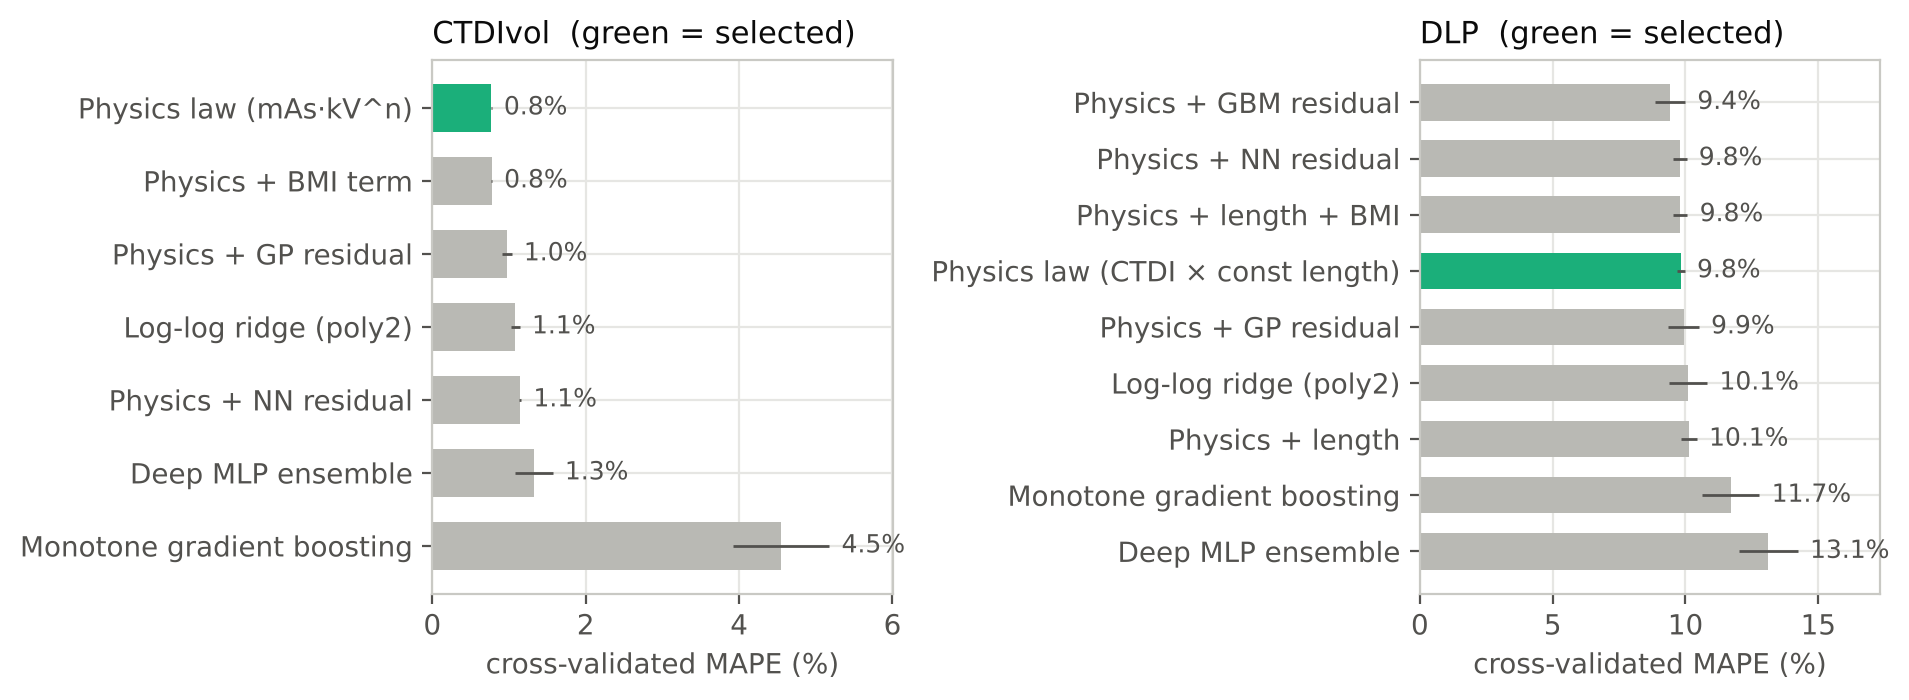
\includegraphics[width=0.88\linewidth]{figs/f2_benchmark.png}
\end{center}
\vspace{2mm}
\begin{itemize}
  \item All models tested the same way: cross-validation, repeated 10 times.
  \item The physics model is the most accurate: \textbf{0.9\%} error for CTDIvol, \textbf{8.2\%} for DLP.
  \item The neural network was worse (2.3\% and 12.4\%). With 50 scans and a known formula, this is expected.
\end{itemize}
\end{frame}

% ---------------- 7 ----------------
\begin{frame}{How accurate is it?}
\begin{columns}[T]
\begin{column}{0.54\textwidth}
  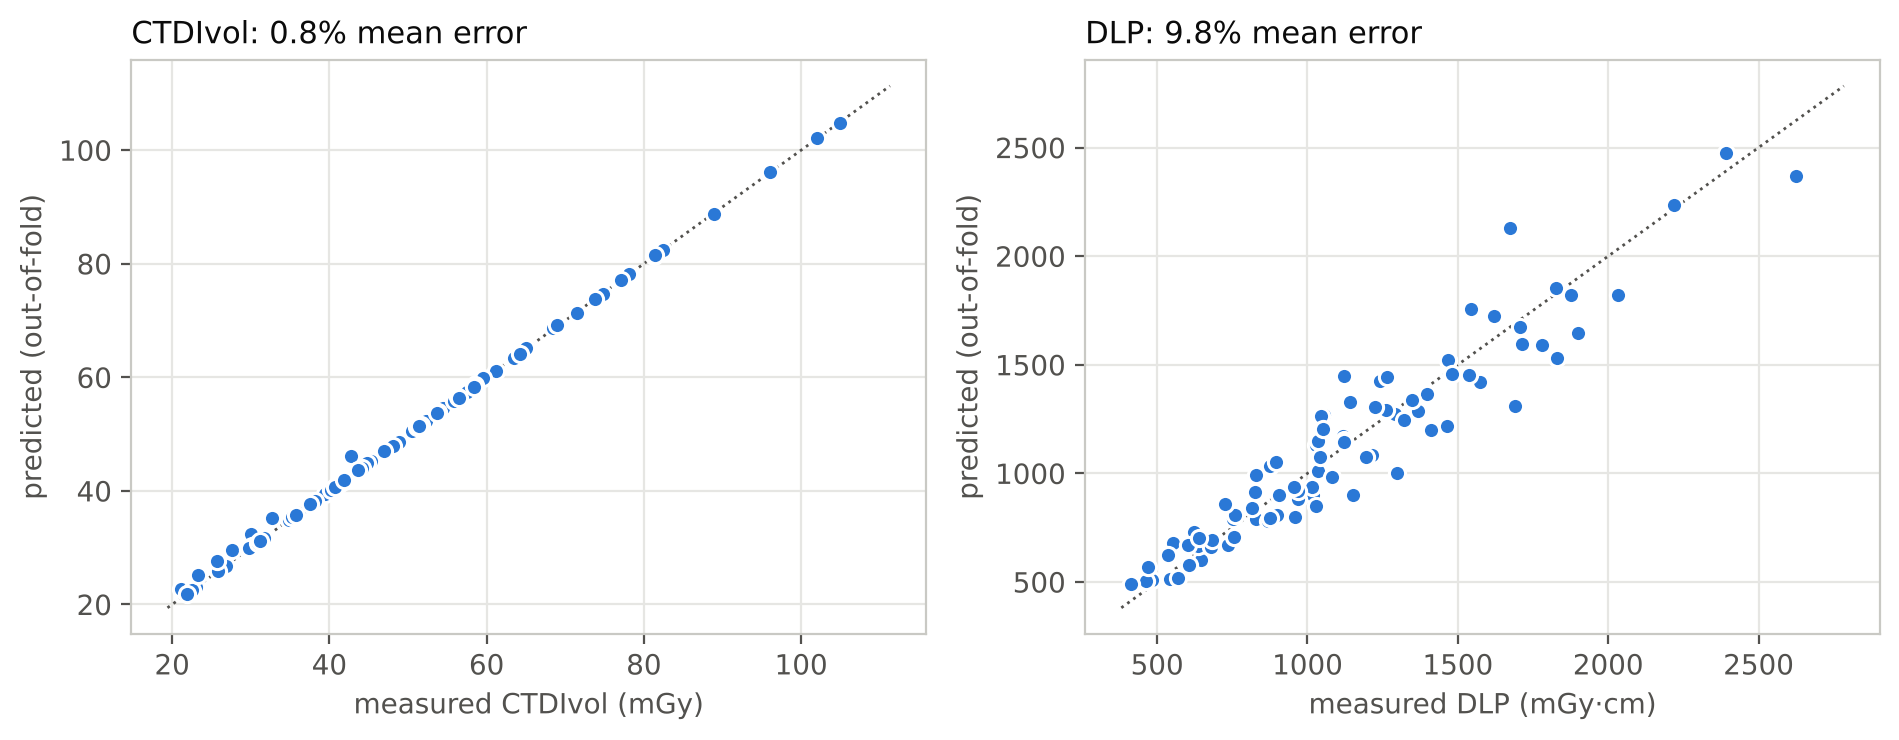
\includegraphics[width=\linewidth]{figs/f3_oof.png}
\end{column}
\begin{column}{0.44\textwidth}
\begin{itemize}\itemsep6pt
  \item Each point was predicted by a model that had not seen it.
  \item CTDIvol is almost perfect.
  \item DLP has more spread. The reason is that the real scan length is not in the data.
  \item Every prediction also comes with a range (90\%), not only a single number.
\end{itemize}
\end{column}
\end{columns}
\end{frame}

% ---------------- 8 ----------------
\begin{frame}{A problem I found in the data}
\vspace{2mm}
\begin{itemize}\itemsep8pt
  \item DLP divided by CTDIvol gives the length that was really irradiated: about \textbf{23 cm}.
  \item But the column called ``SCAN SIZE CM'' does not match it.
  \item That column follows the \textbf{BMI} instead (correlation 0.89), so it is probably the patient size or the
  field of view.
\end{itemize}
\vspace{6mm}
\textbf{Why it matters:} almost all of the 8\% error in DLP comes from this missing information.
If we get the real scan length, the error should drop a lot.
\end{frame}

% ---------------- 9 ----------------
\begin{frame}{How to lower the dose}
\vspace{1mm}
Two simple physics facts:
\begin{center}
noise $\propto 1/\sqrt{\mathrm{dose}}$ \qquad\qquad iodine contrast $\propto \mathrm{kV}^{-1.35}$
\end{center}
\vspace{3mm}
\begin{itemize}\itemsep6pt
  \item Lower kV means more contrast from the iodine, so we can use less dose for the same image quality.
  \item The program searches kV, mAs and scan length, and keeps the estimated image quality the same.
  \item Safety rules: minimum kV depending on BMI, maximum mAs of the tube, and a comparison with what was used
  for similar patients in the same department.
\end{itemize}
\end{frame}

% ---------------- 10 ----------------
\begin{frame}{Example: a typical patient}
\vspace{1mm}
\begin{center}
\begin{tabular}{lrr}
\toprule
 & \textbf{Now} & \textbf{Suggestion} \\
\midrule
kV & 120 & 100 \\
mAs & 756 & 735 \\
Scan length (cm) & 29.8 & 27.8 \\
\midrule
CTDIvol (mGy) & 45.7 & \textbf{28.0} \ ($-39\%$) \\
DLP (mGy$\cdot$cm) & 1056 & \textbf{609} \ ($-42\%$) \\
Estimated image quality & 100\% & 100\% \\
\bottomrule
\end{tabular}
\end{center}
\vspace{5mm}
{\color{mygrey}The program also warns that 100 kV does not exist in our data, so this estimate comes from the
physics formula and should be checked on a phantom first.}
\end{frame}

% ---------------- 11 ----------------
\begin{frame}{The application}
\begin{columns}[T]
\begin{column}{0.42\textwidth}
\textbf{How to use it:}
\begin{enumerate}\itemsep5pt
  \item Type BMI, kV, mAs, scan length.
  \item Read CTDIvol and DLP with their range.
  \item Open ``Reduce dose'' to see the suggestions.
\end{enumerate}
\vspace{4mm}
{\color{mygrey}Written in Python (Streamlit). It runs on a normal PC, offline. Patient data stays on the computer.}
\end{column}
\begin{column}{0.56\textwidth}
  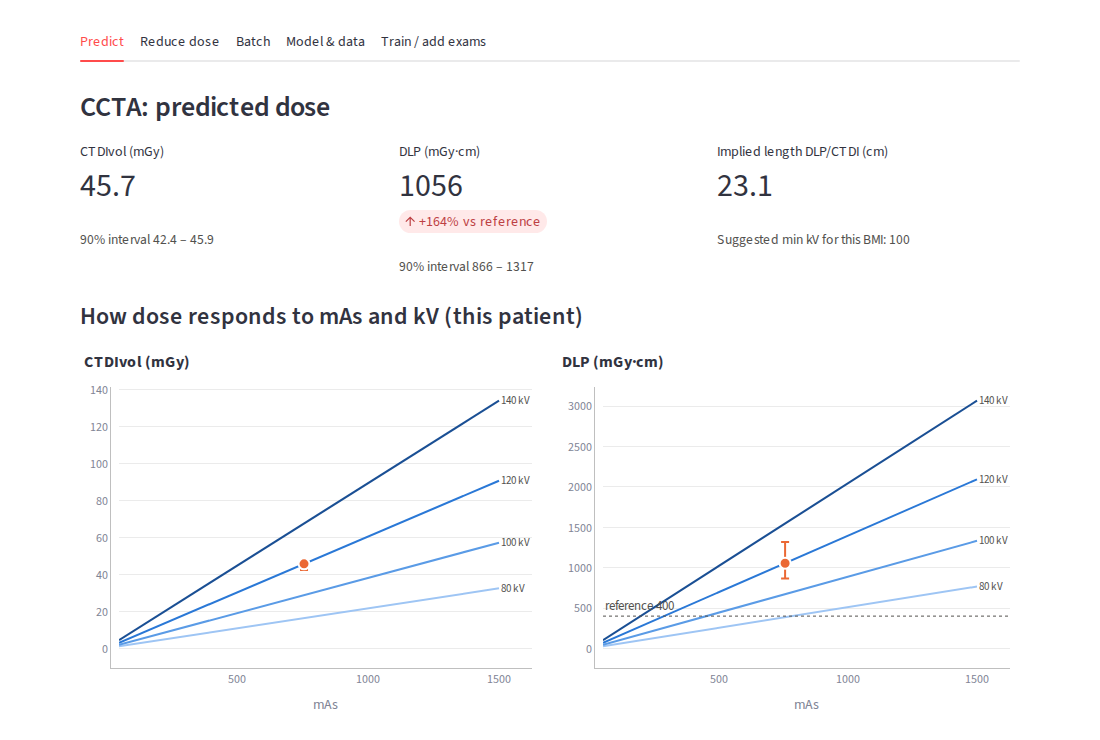
\includegraphics[width=\linewidth]{figs/app_predict.png}
\end{column}
\end{columns}
\end{frame}

% ---------------- 12 ----------------
\begin{frame}{What else is in the program}
\begin{itemize}\itemsep8pt
  \item \textbf{Before the scan:} from the BMI alone it estimates what mAs the machine will choose, and the dose.
  Less accurate, but it works before the patient is on the table.
  \item \textbf{Phantom mode:} it proposes which settings to test on a phantom, you enter the measured image
  quality, and after about 10 scans it finds the lowest dose that is still acceptable.
  \item \textbf{Learning from the radiologists:} the doctor scores each image from 1 to 4, and the program slowly
  learns the lowest dose that is still diagnostic. Every suggestion is approved by a doctor first.
  \item \textbf{Other examinations:} a new file with a different examination gets its own model.
\end{itemize}
\end{frame}

% ---------------- 13 ----------------
\begin{frame}{Limitations and next steps}
\begin{columns}[T]
\begin{column}{0.48\textwidth}
\textbf{Limitations}
\begin{itemize}\itemsep4pt
  \item Only 50 scans, one machine, one examination.
  \item 80 and 100 kV are not in the data, so these values are an extrapolation.
  \item The image quality model is simple and needs to be checked with measurements.
  \item This is a research tool, not a medical device.
\end{itemize}
\end{column}
\begin{column}{0.48\textwidth}
\textbf{Next steps}
\begin{itemize}\itemsep4pt
  \item Ask for the real scan length and the rest of the protocol (dose reports from the scanner).
  \item More examinations, and other types of CT.
  \item Measurements on a phantom with the medical physicist.
  \item A small pilot with a few patients, with the radiologist scoring the images.
\end{itemize}
\end{column}
\end{columns}
\vspace{6mm}
\begin{center}\large Thank you. Questions?\end{center}
\end{frame}

\end{document}
